\documentclass[13pt]{beamer}
\usepackage{beamerthemeshadow}
\usepackage{graphicx}
\graphicspath{ {./images/} }
\usepackage{multirow}
\usepackage{color}
\usepackage[utf8]{inputenc}
\usepackage[T2A]{fontenc} 
\usepackage{hyperref}
\usepackage[flushleft]{threeparttable}
\usepackage[english, serbian]{babel}
\usepackage{graphicx} % Required for inserting images
\definecolor{UBCblue}{rgb}{0.04706, 0.13725, 0.26667}
\usecolortheme[named=UBCblue]{structure}


\setbeamertemplate{navigation symbols}{}
\setbeamertemplate{footline}[frame number]

\usetheme{Copenhagen}
\title{Dajsonova sfera}
\subtitle{-- Teorijski koncept svemirske megastrukture --}
\author{Dimitrije Vujko}
\institute{Matematički fakultet,\\ Univerzitet u Beogradu}
\date{
	\footnotesize{Decembar, 2023.}	
}



\begin{document}

\maketitle



\begin{frame}
	\frametitle{Pregled} % Table of contents slide, comment this block out to remove it
	\tableofcontents[hidesubsections] 
\end{frame}



\section{Upotreba energije}

\begin{frame}{Upotreba energije kroz istoriju}

\begin{itemize}
    \item Ljudsko telo kao glavni izvor energije
    \item Otkriće vatre (pre oko 2 miliona godina)
    \item Industrijalizacija
    \item Atomsko doba (Prva potpuno veštačka nuklarna reakcija 1932. godine)
    \item Dašnji izvori energije
    \begin{itemize}
        \item Nafta 31.2\%
        \item Ugalj 27.2\%
        \item Prirodni gas 24.7\%
        \item Hidro izvori 6.9\%
        \item Nulkearni izvori 4.3\%
        \item Ostali 5.7\%
    \end{itemize}
\end{itemize}

\end{frame}



\section{Kardaševa skala}

\subsection{Tipovi civilizacija}

\begin{frame}{Tipovi civilizacija}

\begin{block}{Definicija}
Kardaševa skala je metod za merenje tehnološkog napretka neke civilizacije.
\end{block}

\begin{itemize}
    \item Nikolaj Kardašev  (russ.~{\em Николай Семёнович Кардашёв})
    \item Godine 1964. definisao \textbf{tri} tipa civilizacije
    \item Merilo tipa civilizacije predstavlja količina potrošive energije
\end{itemize}

\end{frame}


\begin{frame}{Tipovi civilizacija}


\begin{block}{Tip 1}
Civilizacija tipa 1 je u mogućnosti da u potpunosti iskoristi svu energiju svoje planete.
\end{block}

\begin{block}{Tip 2}
Civilizacija tipa 2 je u mogućnosti da iskoristi svu energiju svoje najbliže zvezde.
\end{block}

\begin{block}{Tip 3}
Civilizacija tipa 3 je u mogućnosti da iskoristi svu energiju svoje domaće galaksije.
\end{block}

\end{frame}

\begin{frame}{Kardaševa skala}

    \begin{figure}
        \centering
        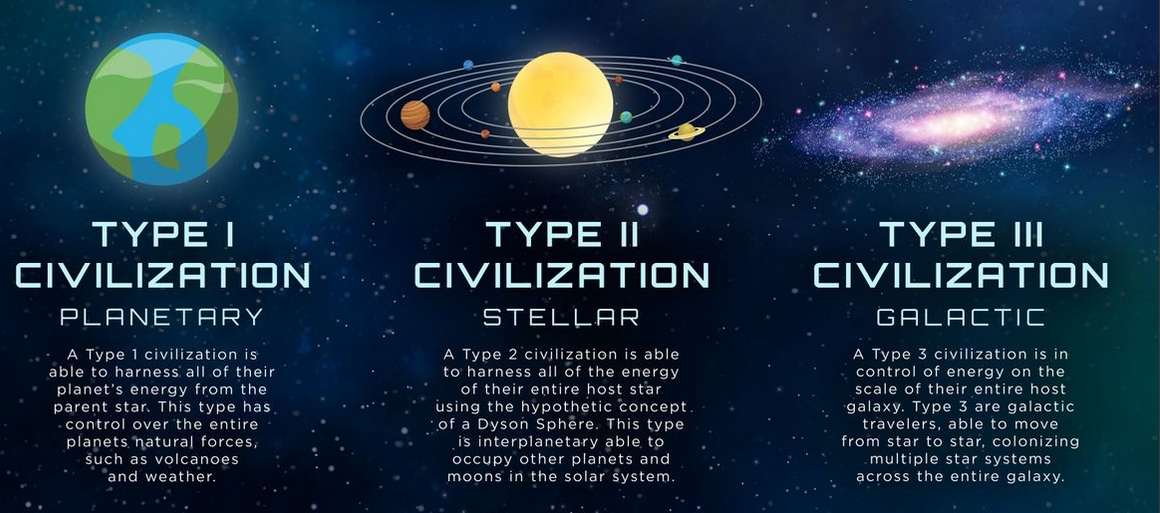
\includegraphics[width=10.5cm, height=4.5cm]{images/Kardaseva skala.png}
        \caption{Kardaševa skala}
        \label{fig:Slika}
    \end{figure}
    
\end{frame}

\begin{frame}{Potrošnja energije}

\renewcommand{\arraystretch}{1.5}
\begin{table}[]
    \centering
    \begin{tabular}{ |p{3cm}||p{3cm}|p{3cm}|  }
        \hline
        Tip 1& Tip 2 & Tip 3\\
        \hline
        $\approx 1 \cdot 10^{16} W$  & $\approx 4 \cdot 10^{26} W$ &$\approx 4 \cdot 10^{36} W$ \\
        \hline
    \end{tabular}
    \caption{Energetska potrošnja tipova civilizacija}
    \label{tab:my_label}
\end{table}

\begin{itemize}
    \item $1 W = 1\frac{J}{s}$ \textit{(Jedan vat je jednak jedan džul po sekundi)}
    \item Potrošnja naše civilizacije u 2020 je bila $2 \cdot 10^{13}W$
    \item Prema Kardaševom modelu, naša civilizacija je tipa 0.73 (u 2020).
\end{itemize}

\end{frame}

\subsection{Šta će se desiti nakon dostizanja civilizacije Tipa 1?}

\begin{frame}{Šta će se desiti nakon dostizanja civilizacije Tipa 1?}


\begin{columns}
    \column{0.5\textwidth}
        \begin{itemize}
        \item Resursi na našoj planeti više nisu dovoljni
        \item Potreba za drugim izvorima energije
        \item Rast populacije
        \item Ukupna količina energije koja se oslobadja iz Sunca svake sekunde iznosi $3.8 \cdot 10^{26} $J


        \item Dajsonova sfera 
        \end{itemize}
        \column{0.5\textwidth}
            \begin{figure}
                \centering
                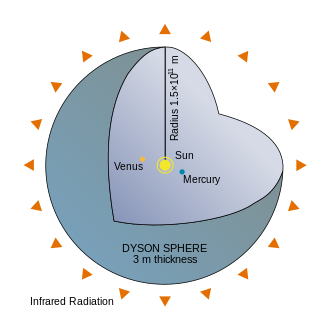
\includegraphics[width=4.5cm, height=4.3cm]{images/Dajsonova sfera.png}
                \caption{Dajsonova sfera (prvobitni koncept)}
            \end{figure}
\end{columns}

\end{frame}






\section{Dajsonova sfera}

\subsection{Koncept Dajsonove sfere}

\begin{frame}{Fridman Dajson}


\begin{columns}
    \column{0.5\textwidth} 
    \begin{itemize}
        \item Rodjen u Velikoj Britaniji 1923. godine
        \item Objavio članak pod nazivom \textit{""Search for Artificial Stellar Sources of Infrared Radiation"}
        \item Dajsonova sfera
        \item Značaj u naučnom svetu i naučnoj fikciji (Star Trek)
        \end{itemize}
    \column{0.5\textwidth}
        \begin{figure}
            \centering
            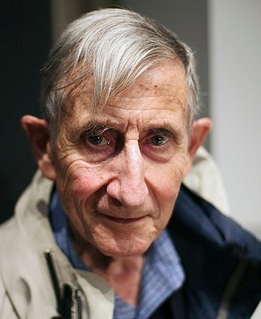
\includegraphics[width=3.5cm, height=3.2cm]{images/fridman dajson.png}
            \caption{eng.~{\em Fridman Dyson}}
        \end{figure}
\end{columns}


\end{frame}


\subsection{Tipovi Dajsonovih sfera}

\begin{frame}{Tipovi Dajsonovih sfera}

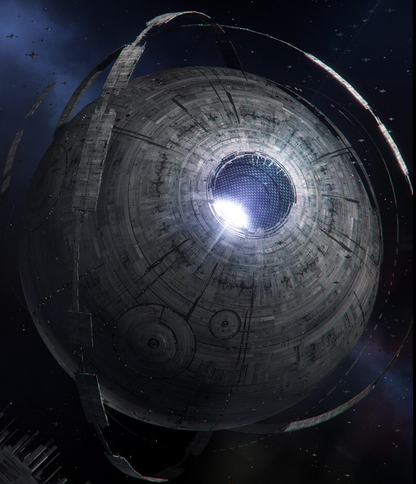
\includegraphics[width=3.5cm, height=4cm]{images/Dajsonova skoljka.png}
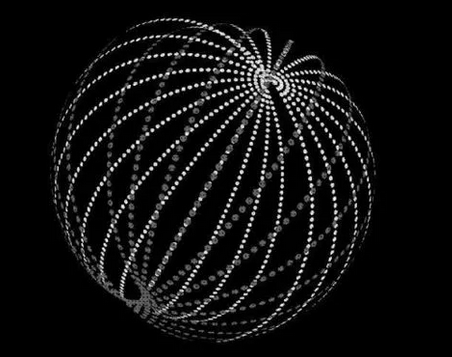
\includegraphics[width=3.5cm, height=4cm]{images/Dajsonov roj.png}
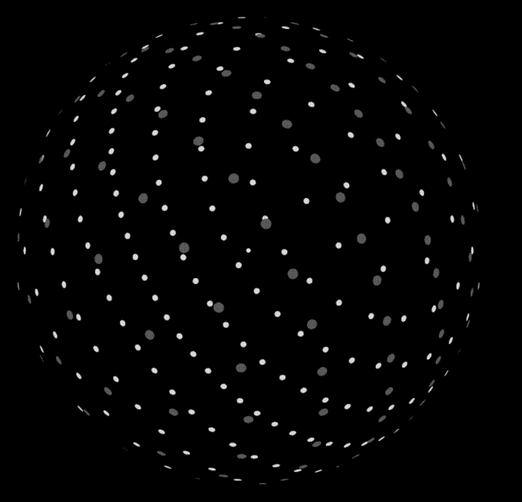
\includegraphics[width=3.5cm, height=4cm]{images/Dajsonov mehur.png}

\begin{itemize}
    \item Dajsonova školjka, Dajsonov roj, Dajsonov mehur
\end{itemize}

\end{frame}

\subsection{Struktura Dajsonove sfere}

\begin{frame}{Kako napraviti Dajsonovu sferu?}

\begin{columns}
    \column{0.6\textwidth}
            Serija koraka za završetak Dysonovog roja prema Stuartu Armstrongu (eng.~{\em Stuart Armstrong}) (pod uslovom da imamo tehnologiju da kolonijalizujemo Merkur):
        \begin{enumerate}
            \item Solarni sakupljači (potrebno $3 \cdot 10^{16}$)
            \item Rudarenje
            \item Rafinerija
            \item Konstrukcija
            \item Lansiranje \textit{(railgun)}
            \item Montaža
        \end{enumerate}
    \column{0.4\textwidth}
        \begin{figure}
            \centering
            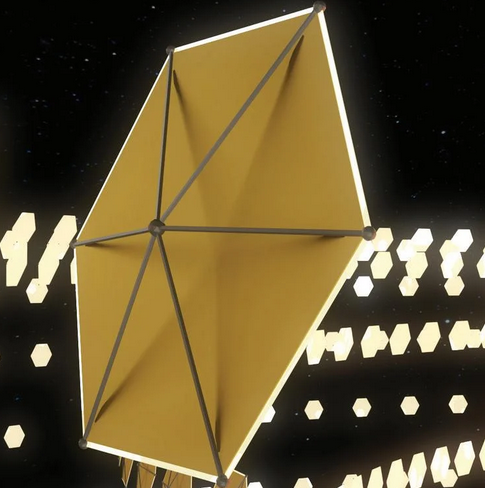
\includegraphics[width=4cm, height=3.5cm]{images/solarni kolektori.png}
            \caption{Solarni sakupljač}
            \label{fig:enter-label}
        \end{figure}
\end{columns}

\end{frame}

\begin{frame}{Dajsonov roj}

\begin{figure}
    \centering
    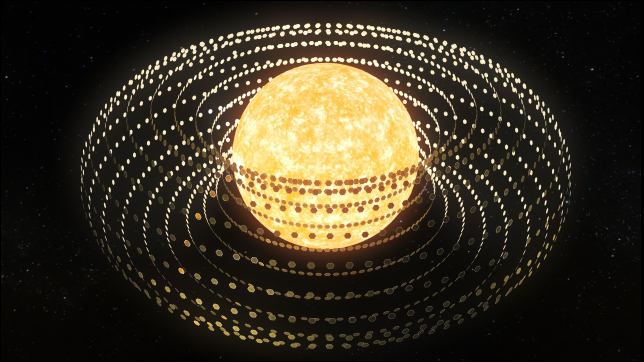
\includegraphics[width=10.5cm, height=5cm]{images/Dajsnonov_roj-2.png}
    \caption{Dajsonov roj}
\end{figure}
    
\end{frame}

\section{Zaključak}

\begin{frame}{Zaključak}

\begin{columns}
    \column{0.6\textwidth}
        \begin{itemize}
            \item Iako izgradnja Dajsonove sfere nosi sa sobom tehnološke izazove, važno je pažljivo razmotriti i etičke i moralne aspekte ovakvog poduhvata.
            \item Izgradnja ovakve strukture znači prelazak u doba neiscrpive energije.
            \item Napredak civilizacije
        \end{itemize}
    \column{0.4\textwidth}
        \begin{figure}
            \centering
            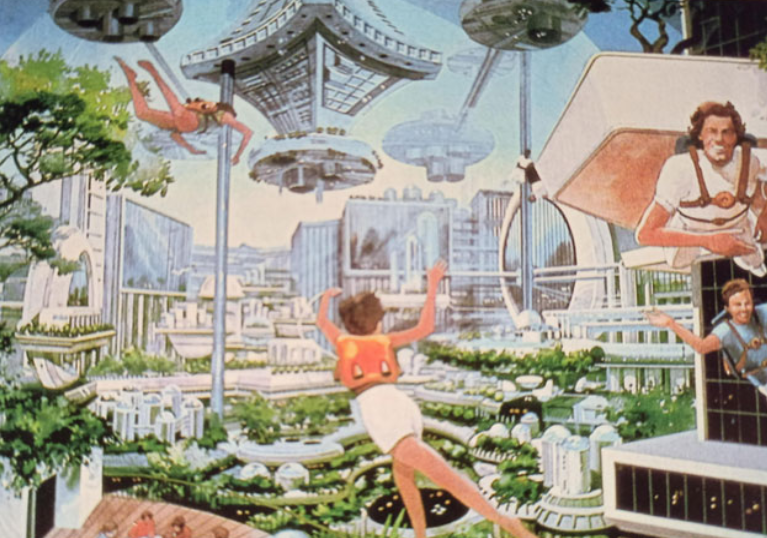
\includegraphics[width=4.2cm, height=4cm]{images/buducnost.png}
            \caption{Budućnost 1959.}
        \end{figure}
\end{columns}

\end{frame}




\section{Literatura}

\begin{frame}{Literatura}

\begin{itemize}
    \item F. J. Dyson, ”Search for Artificial Stellar Sources of Infrared Radiation”
Science, 131, 1667-1668 (1960)
    \item RealClear Science, "How to Build a Dyson Swarm" by Ross Pomeroy
    (\url{https://www.space.com/38031-how-to-build-a-dyson-swarm.html})
    \item Ibrahim Semiz and Salim Ogur, Bogazici University, Department of Physics Bebek, ˙Istanbul, TURKEY, "Dyson Spheres around White Dwarfs", March 2015.
\end{itemize}

\end{frame}


\begin{frame}

\begin{center}
    \textbf{HVALA NA PAŽNJI!}
\end{center}

\end{frame}

\end{document}

